\documentclass[11pt,a4paper]{article}
\usepackage{fontspec}
\setmainfont{Source Serif 4}[Path=/home/claude/ref/fonts/, UprightFont=SourceSerif4-Regular.ttf, BoldFont=SourceSerif4-Semibold.ttf, ItalicFont=SourceSerif4-It.ttf]
\setmonofont{IBM Plex Mono}[Path=/home/claude/ref/fonts/, UprightFont=IBMPlexMono-Regular.ttf, BoldFont=IBMPlexMono-Medium.ttf, Scale=0.88]
\usepackage[a4paper,margin=2.4cm]{geometry}
\usepackage{amsmath}
\usepackage{graphicx,booktabs,float,caption,array,xcolor,longtable}
\usepackage{xurl}
\usepackage[hidelinks]{hyperref}
\usepackage[round]{natbib}
\usepackage{setspace}
\setstretch{1.08}
\renewcommand{\topfraction}{0.9}
\renewcommand{\bottomfraction}{0.8}
\renewcommand{\textfraction}{0.1}
\renewcommand{\floatpagefraction}{0.75}
\setlength{\parindent}{0pt}
\setlength{\parskip}{0.55em}
\captionsetup{font=small,labelfont=bf}
\setlength{\bibsep}{3pt}
\urlstyle{same}
\hypersetup{pdftitle={Where Slavery Money Came Home},pdfauthor={Dr Tristan Hotham}}

\begin{document}
\begin{center}
{\Large\bfseries Where Slavery Money Came Home: The British Addresses of Slave-Owners and Compensation Claimants at Abolition, Mapped from the Legacies of British Slavery Database\par}
\vspace{1.2em}
{\large Dr Tristan Hotham\par}
\vspace{0.3em}
{\small Independent researcher\\
ORCID: 0000-0003-4931-9349\\
DOI: https://doi.org/10.5281/zenodo.24113858\par}
\vspace{0.8em}
2026
\end{center}

\begin{quote}
\small
\begin{center}\textbf{Abstract}\end{center}
When Britain abolished colonial slavery in 1833 it paid \pounds 20 million in compensation to slave-owners and nothing to the people they had enslaved. The Legacies of British Slavery (LBS) database at University College London has traced many of the owners and claimants to addresses in Britain. Its own map warns that it is a search tool and not yet data for statistical analysis. Taking that warning seriously, this paper describes the geography of the 3,187 geocoded LBS addresses in Great Britain against the 1831 census, using a plan written before the analysis. London holds 36\% of the addresses; Middlesex holds 33\% against 8\% of the population, and the county Gini coefficient is 0.51 (95\% CI 0.50 to 0.53). Per head, Scotland (2.06 per 10,000) matches England (2.04) and Wales is far lower (0.51). In a Poisson model across 84 counties, each doubling of distance from the nearest of London, Bristol, Liverpool and Glasgow goes with a 37\% lower rate (95\% CI 25 to 46\%); the pattern is carried by street addresses, is not robust to leaving out the South-East region, and listed great houses, a proxy for landed wealth, show none. Outside London, 28\% of addresses are named houses, and an estimated 44\% of country-house addresses are listed buildings today. The results describe a database, not a census, and they are associations only.

\textbf{Keywords:} slavery compensation; slave-ownership; Legacies of British Slavery; historical geography; country houses; Britain; 1830s
\end{quote}

\section{Introduction}\label{sec:intro}
The Slavery Abolition Act of 1833 ended slavery in most of Britain's colonies from 1 August 1834. It did so on terms set by and for the owners. Most of the people it freed were bound to work without pay for their former owners as ``apprentices'', a system abolished in the British West Indies on 1 August 1838 \citep{baker2024,holt1992}. Parliament voted \pounds 20 million to compensate the owners for the loss of what the law treated as their property, a sum equal to about 40\% of government spending in 1833 \citep{baker2024}. ``The formerly enslaved population received no compensation'' \citep{baker2024}. Arguments about who benefited from slavery, and about what is owed, have turned on this asymmetry ever since \citep{williams1944,beckles2013}.

The records of the Slave Compensation Commission, which handled the claims, provide what the Legacies of British Slavery project calls ``a more or less complete census of slave-ownership in the British Empire in the 1830s'' \citep{lbs2026details}. Since 2009 the project at University College London has used them, with wills, directories, newspapers and family papers, to trace the owners, claimants and beneficiaries, with ``a particular emphasis on the `absentee' owners based in Britain'' \citep{lbs2026details,draper2010,hall2014}. One product is a map of the British addresses of the people in the database. The LBS team are clear about what it is: ``This map is a search tool and a general guide. More work is needed to produce data for statistical analysis'' \citep{lbs2026maps}.

This paper takes that caveat as its starting point rather than an obstacle. It asks a descriptive question that the address file can answer, provided its limits are stated: where in Britain did the people linked to slave-ownership at abolition live, relative to the population of the time? It sets the 3,187 geocoded addresses in Great Britain against county populations from the 1831 census, asks how concentrated they are, whether they follow the geography of the Atlantic ports, how many are town houses and how many country seats, and how many of those country seats survive as listed buildings today. The analysis plan was written before any rate, model or match was computed, and the paper reports the planned results first.

I hope three things are new. First, the paper gives a per-capita county geography of the geocoded LBS addresses for the whole of Great Britain, with intervals, and shows that the bulk of the concentration is metropolitan. Second, it tests a simple spatial hypothesis, that addresses thin out with distance from the four great West India ports, and finds a gradient that is carried by town addresses and depends on London and the South-East (it loses statistical support when that region is left out), while country houses are spread without regard to distance, as are listed great houses in a placebo comparison. Third, it links the country-house addresses to today's national lists of listed buildings with a hand-checked matching rule, which gives a first estimate of how much of this built inheritance is protected and visible. Throughout, the subject of the data is the owners; the people whose labour and lives produced the wealth appear in these records, as the LBS team put it, without ``systematic information on the enslaved themselves'' \citep{lbs2026details}. The paper does not try to measure the harm of slavery, and nothing in it should be read as doing so.

Section~\ref{sec:lit} reviews the work on slave-ownership and compensation in Britain. Section~\ref{sec:data} describes the data and Section~\ref{sec:design} the plan. Section~\ref{sec:results} reports the results and Section~\ref{sec:robust} the checks. Section~\ref{sec:disc} discusses what the pattern means and what the data cannot show.

\section{Background and literature}\label{sec:lit}
\subsection{Slavery, compensation and British wealth}
The question of how far British prosperity rested on slavery is old and contested. \citet{williams1944} argued that the profits of slavery and the slave trade helped finance industrialisation and that abolition followed when the system stopped paying. Critics replied that the profits were too small a share of national investment to matter much; \citet{eltis2000} judged the contribution of slavery and the trade to industrialising Britain to be real but modest. \citet{inikori2002} placed African and Atlantic markets at the centre of English industrial growth. More recently \citet{heblich2022} combined the compensation records with a spatial model and concluded that slavery wealth shifted local economies away from agriculture and towards manufacturing, and raised local incomes most in the places most involved.

Compensation itself became a subject of study only with the opening of the Commission's records to systematic work. \citet{butler1995} studied how the compensation was distributed in Jamaica and Barbados, among planters, merchants and creditors. \citet{draper2007,draper2010} reconstructed the British side of the compensation: who claimed, through which agents, and how slave-ownership and the claims were woven into metropolitan society. \citet{hall2014} widened this into a study of the legacies of slave-ownership across commerce, politics, culture, physical remains and historical writing in Victorian Britain. \citet{draper2008} traced the slave-owning connections of the City's first dock companies. The present paper uses the addresses that this body of work produced; it adds no new archival evidence about any person.

\subsection{Places: ports, cities and country houses}
Much of the literature is organised by place. Bristol \citep{dresser2001}, Liverpool \citep{richardson2007} and Glasgow \citep{mullen2022,devine2015} each have a historiography of their Atlantic trade and its people, and London's role as the centre of finance, insurance and absentee ownership runs through \citet{draper2010} and \citet{donington2019}. The universities have examined their own connections \citep{mullen2021}. In historical geography, \citet{seymour1998} showed how one Herefordshire landowner managed an English estate and a Grenada plantation as parts of the same enterprise, and \citet{lambert2005} studied white creole identity and its metropolitan ties. Country houses have been a particular focus, both in scholarship \citep{dresser2013,smith2006} and in the work of heritage bodies; the National Trust's review of its own properties found connections to colonialism and historic slavery at many of them \citep{huxtable2020}.

These studies are mostly local or biographical. There is less work that looks at the whole national pattern of addresses with a common denominator. \citet{heblich2022} use slave-owner wealth by location as an explanatory variable rather than as a pattern to be described, and the LBS map itself shows counts and leaves per-capita comparison to the user. This paper fills that descriptive gap, with care about what the address file is.

\subsection{Counting the compensation}
Most quantitative work on the compensation has counted claims, awards and money. \citet{draper2010} analysed the awardees and claimants, including absentee owners in Britain and the merchants and agents who acted for them. \citet{butler1995} followed the compensation through the planters and creditors of Jamaican and Barbadian estates. \citet{heblich2022} aggregate slave-owner wealth by location to explain later economic change. These studies treat the compensation records as a source of amounts and connections. The address file used here is a different kind of source. It was built to help users find the people and places in the database, and it records residence over a lifetime, often for people who received nothing directly but were heirs, mortgagees or annuitants. Its value is breadth: it covers thousands of people and places across Britain on a common footing. Its weakness is that it was not designed for counting, which is why the LBS team warn against statistical use without further work \citep{lbs2026maps}. The approach taken here is to state that warning, to describe the geocoded subset with denominators and intervals, to check whether the gaps in geocoding are related to the results, and to avoid inferences about money.

\subsection{Heritage and public memory}
The geography of slave-ownership has also become a public question. Heritage bodies and local historians have used the LBS database to find the slavery connections of buildings, streets and institutions, and the results have sometimes been contested in public debate. \citet{dresser2013} brought together research on the country house, showing both the reach of slavery wealth into the English countryside and the difficulty of separating it from other sources of landed income. The \citet{huxtable2020} report documented connections at properties in the care of the National Trust. A national, reproducible link between the LBS addresses and the statutory lists of listed buildings has not, to my knowledge, been published. Such a link cannot settle what a building means, but it can show how many of the recorded houses still stand, which of them the state protects, and where they are.

\subsection{Expectations}
Three expectations follow from this literature. First, the addresses should be concentrated in London, where finance, agents and many absentee owners were \citep{draper2010}. Second, they should be denser near the Atlantic ports through which the West India trade passed. Third, outside the cities many addresses should be country seats, some of which survive as protected buildings \citep{dresser2013}. The second expectation is the one tested formally.

\section{Data}\label{sec:data}
\subsection{The LBS address file}
The LBS map of Britain draws on a file of addresses, each with an OpenStreetMap geocode, the class of the geocoded feature (a building, a street, a settlement or an administrative area), the street text, district, town, county, region and country, and a list of the people in the database linked to it, with start and end years where known \citep{lbs2026maps}. The file used here, retrieved in 2026, has 3,445 rows; 8 have no coordinates. Two rows in St Peter Port, Guernsey, labelled England in the file, are counted with the Channel Islands, and two British addresses geocoded to namesake towns abroad (Ipswich in Queensland and Bath in Kentucky) were moved to the centre of the LBS points for their town and treated as area geocodes. Of those with coordinates, 3,187 are in Great Britain, 80 in Ireland, 13 in the Channel Islands and 157 elsewhere (Table~\ref{tab:flow}). The LBS map page reports 5,686 addresses in the database, of which 3,450 had been located \citep{lbs2026maps}; the LBS county table that accompanies the map lists 5,138 addresses in British counties, of which 3,115 (61\%) are located. In Great Britain the addresses are linked 5,331 times to 4,004 different people; 798 addresses have two or more people and 19 have none listed.

The people are those whom the database links to slave-ownership or to the compensation: owners at abolition, awardees and claimants, and others such as mortgagees and legatees \citep{lbs2026details}. An address is a place where a person lived at some time; the dates are often unknown. Where a year is given (2,876 addresses, 90\%), the median earliest year is 1834 and 71\% fall between 1800 and 1859 (Figure~\ref{fig:dates}). The file holds no compensation amounts, so this paper is about residence, not money.

\begin{figure}[tbp]\centering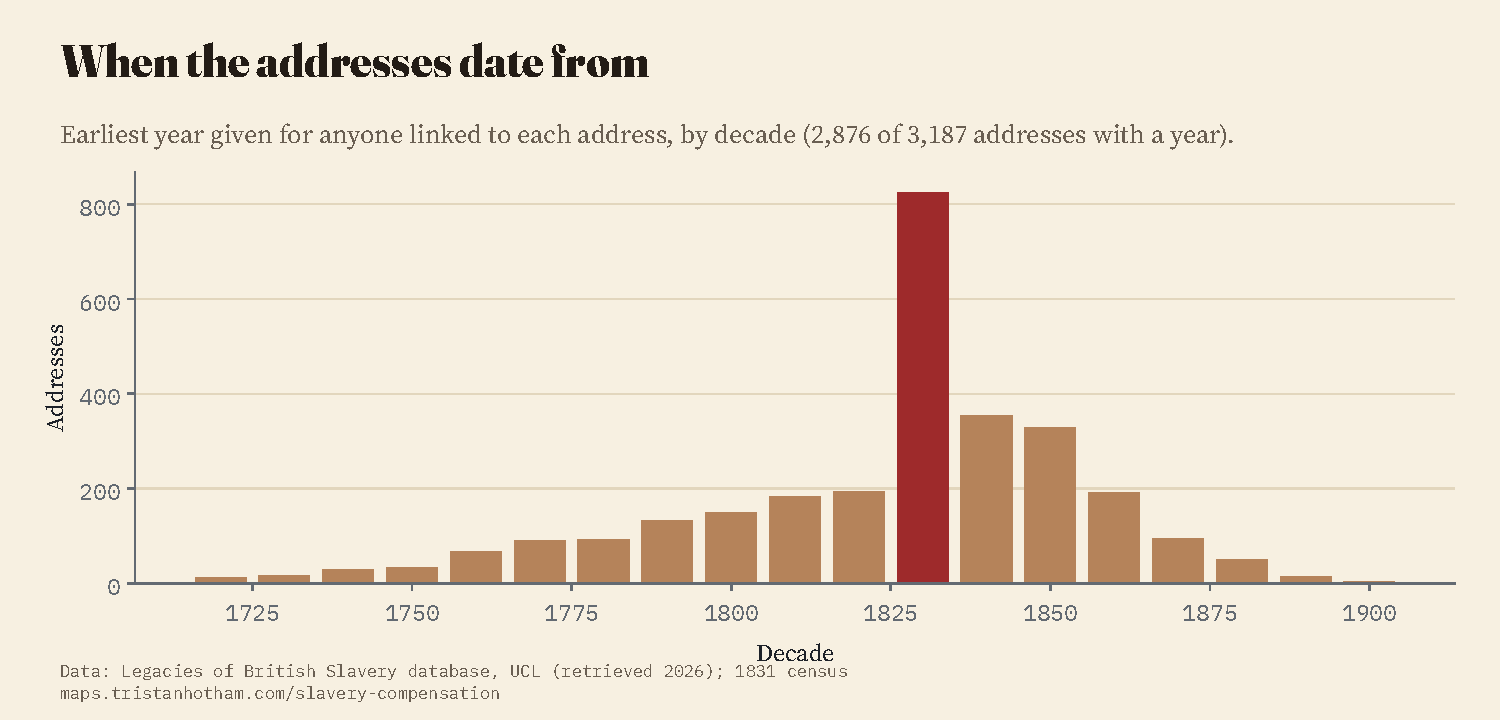
\includegraphics[width=0.85\textwidth]{f_dates.pdf}\caption{Earliest year given for anyone linked to each address, by decade, Great Britain (addresses with a year only).}\label{fig:dates}\end{figure}

The dates show why the addresses should not be read as a snapshot of 1834. The spike in the 1830s reflects the compensation itself, when claims, counterclaims and awards put many people on record at a known place. But the earliest years reach back into the eighteenth century, because the database also records people linked to the same estates before abolition, and forward into the 1860s and later, because some people are known only from later directories, wills or obituaries. A person who lived in Bath in 1840 and London in 1850 contributes two addresses. The county counts are therefore counts of known residences of a population of owners and claimants over a period centred on the 1830s, not a census of where the compensation money was spent.

Personal names are never used or republished. The released data hold counts by county and town, unnamed points with the LBS map identifier and the LBS identifier of one linked record (so that a reader can follow the record to UCL) and the matching decisions for country houses.

\begin{table}[tbp]\centering\small\caption{Data flow.}\label{tab:flow}\begin{tabular}{lr}\toprule Item & Number\\\midrule
Rows in the LBS map address file & 3,445\\
\quad without coordinates & 8\\
\quad Great Britain & 3,187\\
\qquad England & 2,654\\
\qquad Scotland & 487\\
\qquad Wales & 46\\
\quad Ireland & 80\\
\quad Channel Islands & 13\\
\quad elsewhere & 157\\\midrule
Person links, Great Britain & 5,331\\
Distinct people, Great Britain & 4,004\\
LBS county table: all addresses & 5,138\\
\quad located & 3,115\\\midrule
Country-house candidates & 553\\
\quad matched to a listed building & 267\\
\bottomrule\end{tabular}\end{table}

\subsection{Counties and population}
Counties are the historic (pre-1889) counties used in the 1831 census. The LBS county field mostly uses these names; 18 addresses with modern or missing county names were placed by their point, and spelling variants were mapped by hand (all in the code). For England and Wales I checked the LBS county against the county of the nearest 1851 parish centroid \citep{caprettini2020}: they agree for 97.0\% of 2,686 addresses, and the 81 disagreements lie near county borders, most often between Middlesex and Surrey. The LBS county is kept.

\textit{London} is the LBS region ``London'' (the metropolis as LBS defines it, covering parts of Middlesex, Surrey and Kent; 1,150 addresses) together with 8 addresses whose town is given as London or the City of London but which carry another region. The plan defined London by the LBS region alone; the town rule was added after the plan, before the write-up, so that the London count and the London town count agree. No test depends on it.

County populations for 1831 (and 1841, for a check) come from the Census of Great Britain, 1851, Population Tables I, Vol.~I, Tables XXX and X \citep{census1851}, in a transcription \citep{ditto2026} that I checked against the printed totals for England, Wales and Scotland, which it matches exactly. As a second check, the 1831 county figures reprinted in the 1841 census abstract \citep{vob2026} are identical for 52 of the 84 counties and within 1\% for all but six; the six (Durham, Northumberland, Worcestershire, Shropshire, Wiltshire and Denbighshire, 1\% to 6\%) reflect changes to county boundaries between the two reports, and the 1851 figures, on the later boundaries, are used. Yorkshire is the sum of its three ridings and the City of York; Monmouthshire is placed in Wales, as on the LBS map. Ireland is left out of the per-capita work. The LBS county table carries its own population column; it matches the 1841 census within 5\% for 79 of 84 counties, but not for Middlesex, Surrey, Kent, Norfolk and Northamptonshire, and it is not used.

\subsection{Address forms and geocode precision}
Each address is classed from its text as a \textit{street address} (a house number or a street word such as Street, Square, Terrace or Crescent), a \textit{named house} (a named property such as a Hall, Park or Castle, or a bare house name), an \textit{institution} (a college, hospital or asylum) or \textit{settlement only} (no street text, just a town, village or parish). The geocode precision comes from the OpenStreetMap class: the building itself (16\%), the street (50\%) or only an area such as a town or parish (34\%). Several addresses can share a point: 490 share coordinates with another.

\subsection{Listed buildings}
The country-house comparison uses the national lists of listed buildings of England (Historic England), Scotland (Historic Environment Scotland) and Wales (Cadw), harmonised in \citet{hotham2026listed}: each entry's name, grade, broad type and point. For the county comparison, \textit{listed great houses} are Grade I and II* entries of type house in England and Wales whose names contain Hall, House, Park, Court, Castle, Abbey, Manor, Grange, Priory or Place and not an outbuilding word, outside parishes with an 1801 density of 1,000 people per km$^2$ or more \citep{caprettini2020}; there are 5,085.

\section{Research design}\label{sec:design}
\subsection{Analysis plan}
The plan (in the repository as \texttt{NOTES.md}) was written after inspecting the structure of the raw files and before computing any rate, model or match. It fixed the definitions above, the unit (the historic county), the outcome (geocoded addresses, with linked people as an alternative), the main model, the checks and what would count against the hypothesis. The rules for matching country houses to listed buildings were developed on two samples and frozen before the evaluation sample was drawn (Section~\ref{sec:listed}). Analyses added afterwards are marked exploratory.

\subsection{Concentration (Q1)}
I compare shares of addresses and of population for London, Middlesex and the three nations, and compute a population-weighted Gini coefficient of addresses across the 84 counties, with a 95\% interval from 2,000 multinomial resamples of the addresses.

\subsection{Distance from the ports (H2)}
Let $y_c$ be the geocoded addresses in county $c$ and $N_c$ its 1831 population. The main model is a Poisson regression with offset $\log N_c$:
\begin{equation}
\log E[y_c] = \log N_c + \beta_0 + \beta_1\,\mathrm{Port}_c + \beta_2 \log D_c + \beta_3\,\mathrm{Wales}_c + \beta_4\,\mathrm{Scotland}_c,
\end{equation}
where $\mathrm{Port}_c$ marks the counties of the four great West India ports (Middlesex for London, Gloucestershire for Bristol, Lancashire for Liverpool, Lanarkshire and Renfrewshire for Glasgow and Greenock) and $D_c$ is the great-circle distance in km from the county's centre to the nearest of the four city centres (floored at 5 km). County centres are the 1801-population-weighted means of their 1851 parish centroids in England and Wales \citep{caprettini2020} and the county towns in Scotland. Standard errors are heteroskedasticity-robust (HC1), which makes the Poisson estimates valid under over-dispersion \citep{santossilva2006,cameron2013}. $e^{\beta_2 \ln 2}$ is the rate ratio for a doubling of distance. H2 predicts $\beta_2<0$ and $\beta_1>0$; a 95\% interval for $e^{\beta_2}$ including 1 would count against it.

Planned checks: a negative binomial model; linked people instead of addresses; all LBS addresses including the unlocated ones (which tests whether gaps in geocoding drive the result); leaving out Middlesex; England only; Scotland only; the 1841 population as the offset; named houses only and street addresses only; leaving out each LBS region in turn; and a placebo outcome, listed great houses in England and Wales, as a rough stand-in for old landed wealth. If the addresses only tracked landed wealth, the placebo would show the same distance gradient.

\subsection{Town and country (Q3) and country houses (Q4)}\label{sec:listed}
Q3 is descriptive: the shares of each address form in London, the rest of England, Wales and Scotland. As an exploratory check, addresses in England and Wales outside London are called urban if their nearest 1851 parish had an 1801 density of 1,000 people per km$^2$ or more.

For Q4 the candidates are named houses in Great Britain outside London and outside such urban parishes (553). A candidate matches a listed entry within 2 km (5 km for an area geocode) when the distinctive words of the two names (the name without generic words such as house, hall, park or the) agree (fuzzy ratio at least 90, first distinctive word shared), the listed name does not add an outbuilding word (lodge, stables, gate, farm and so on) and the house types do not conflict. The rule was refined on two development samples and then frozen. On a fresh evaluation sample of 50 matches and 50 non-matches, read by eye, 7 matches were wrong or doubtful (precision 86\%) and 2 non-matches were houses that are in fact listed (4\%). The corrected share is precision times the matched share plus the miss rate times the unmatched share, with an interval from binomial resampling of the two rates. By county I compute candidates per 100 listed great houses and its Spearman correlation with the county address rate (H4: positive).

\section{Results}\label{sec:results}
\subsection{Concentration}
Figure~\ref{fig:map} shows the addresses and the county rates. London holds 1,158 addresses, 36.3\% of those in Great Britain. Middlesex holds 33.4\% of the addresses and had 8.4\% of the population, 4.0 times its share (Figure~\ref{fig:shares}). Half of all addresses are in five counties with 24\% of the population, and 4 counties have none. The Gini coefficient across counties is 0.51 (95\% CI 0.50 to 0.53); 0.51 for linked people, 0.53 for all LBS addresses including the unlocated, and 0.42 without Middlesex. The expectation of strong metropolitan concentration holds.

\begin{figure}[tbp]\centering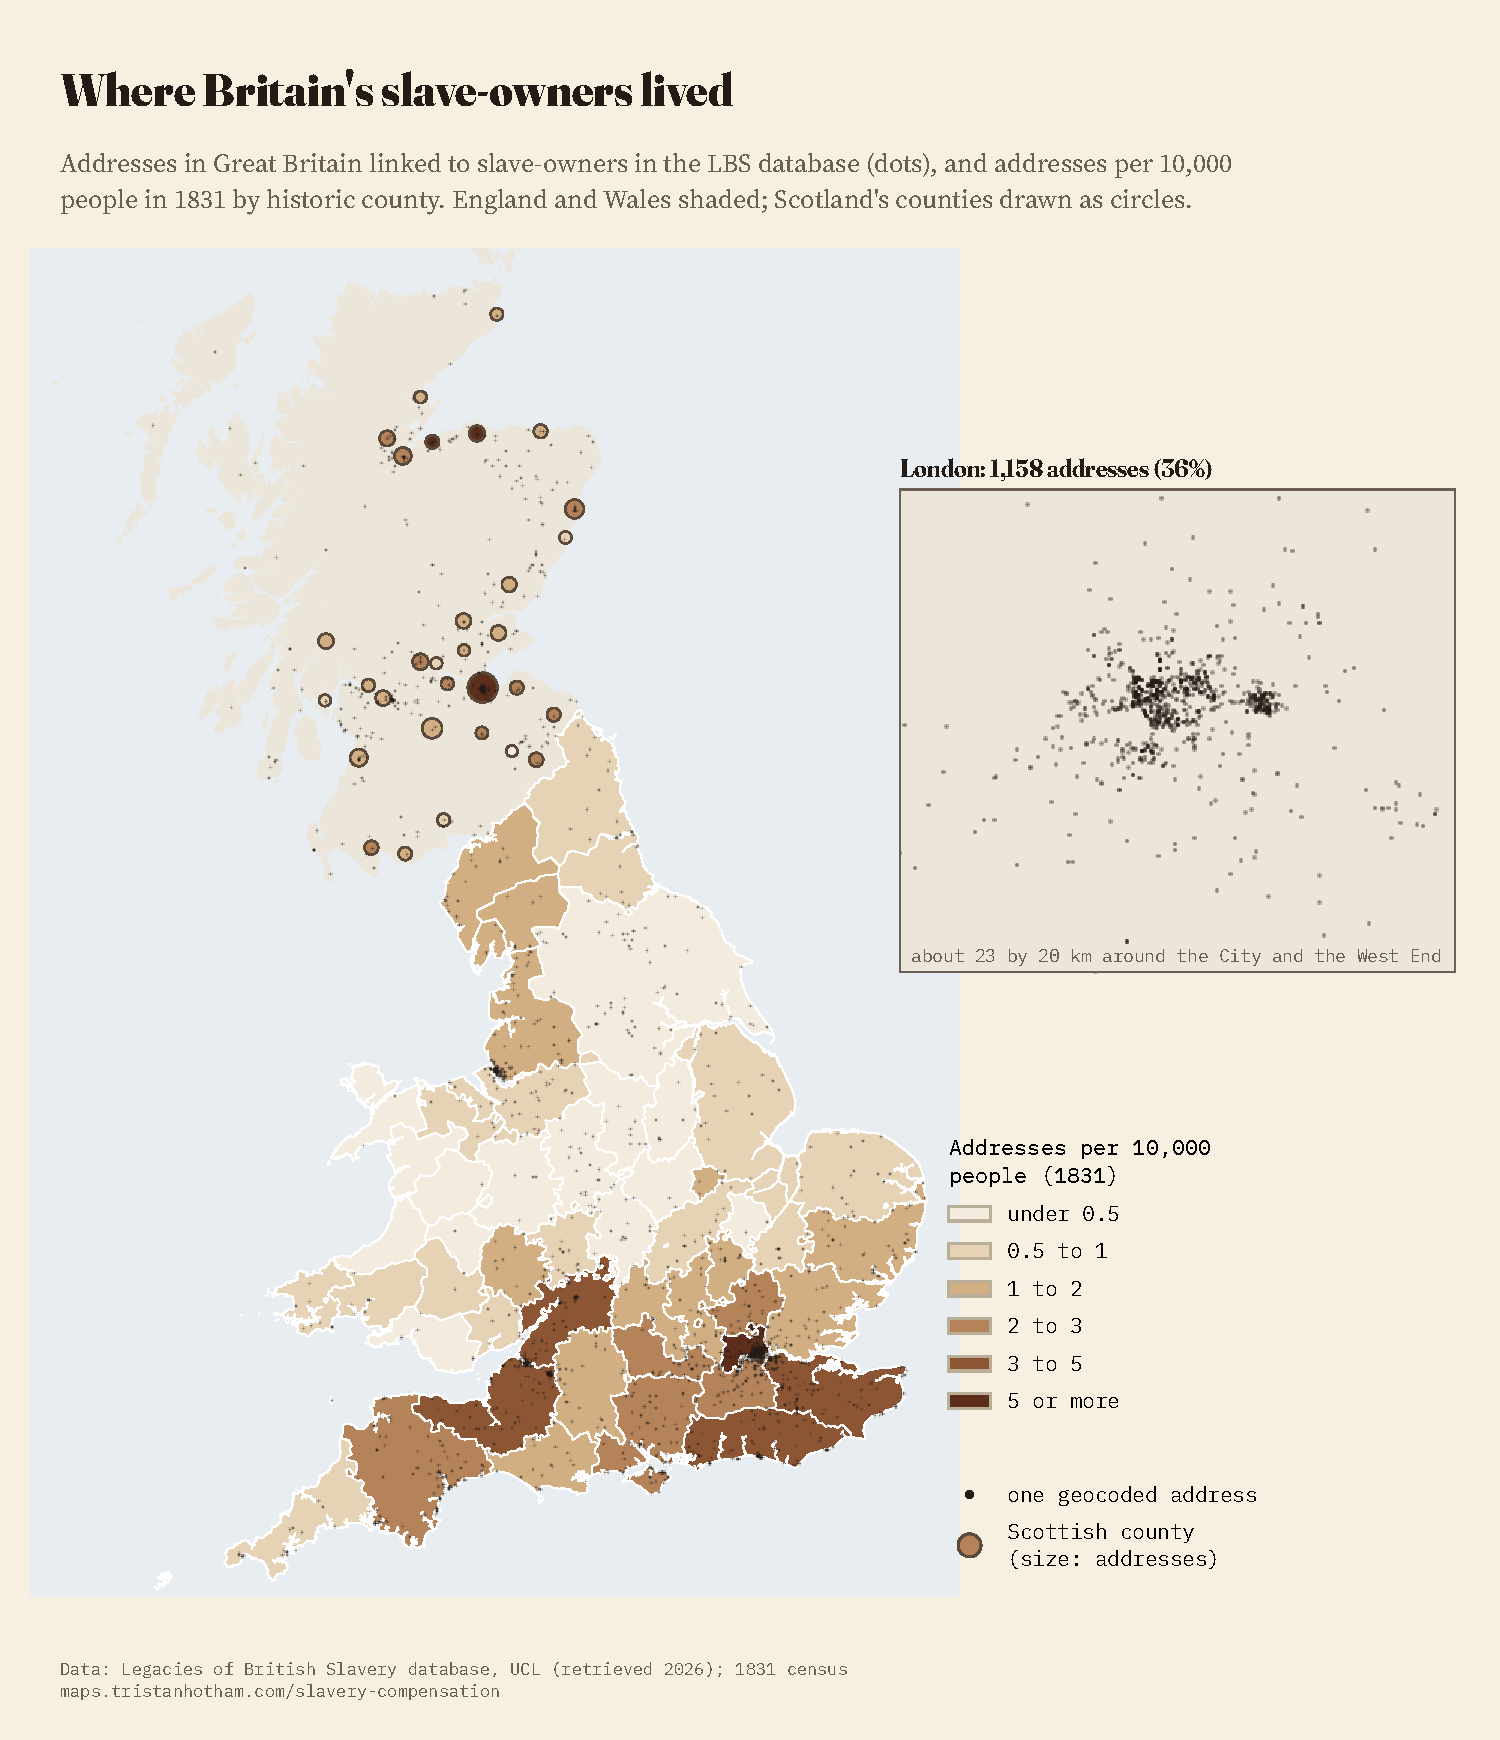
\includegraphics[width=0.92\textwidth]{f_map.pdf}\caption{Geocoded LBS addresses in Great Britain (dots) and addresses per 10,000 people in 1831 by historic county. England and Wales: approximate county outlines rebuilt from 1851 parishes; Scotland: circles at county towns, sized by addresses. Inset: London.}\label{fig:map}\end{figure}

The towns tell the same story (Figure~\ref{fig:towns}). After London (1,158) come Edinburgh (121), Bristol (106), Liverpool (100), Bath (66), Glasgow (32), Brighton (26) and Cheltenham (18); the top five hold 49\% of the addresses. The list mixes the Atlantic ports with the capital cities and the resort and spa towns where people of means lived and retired.

\begin{figure}[tbp]\centering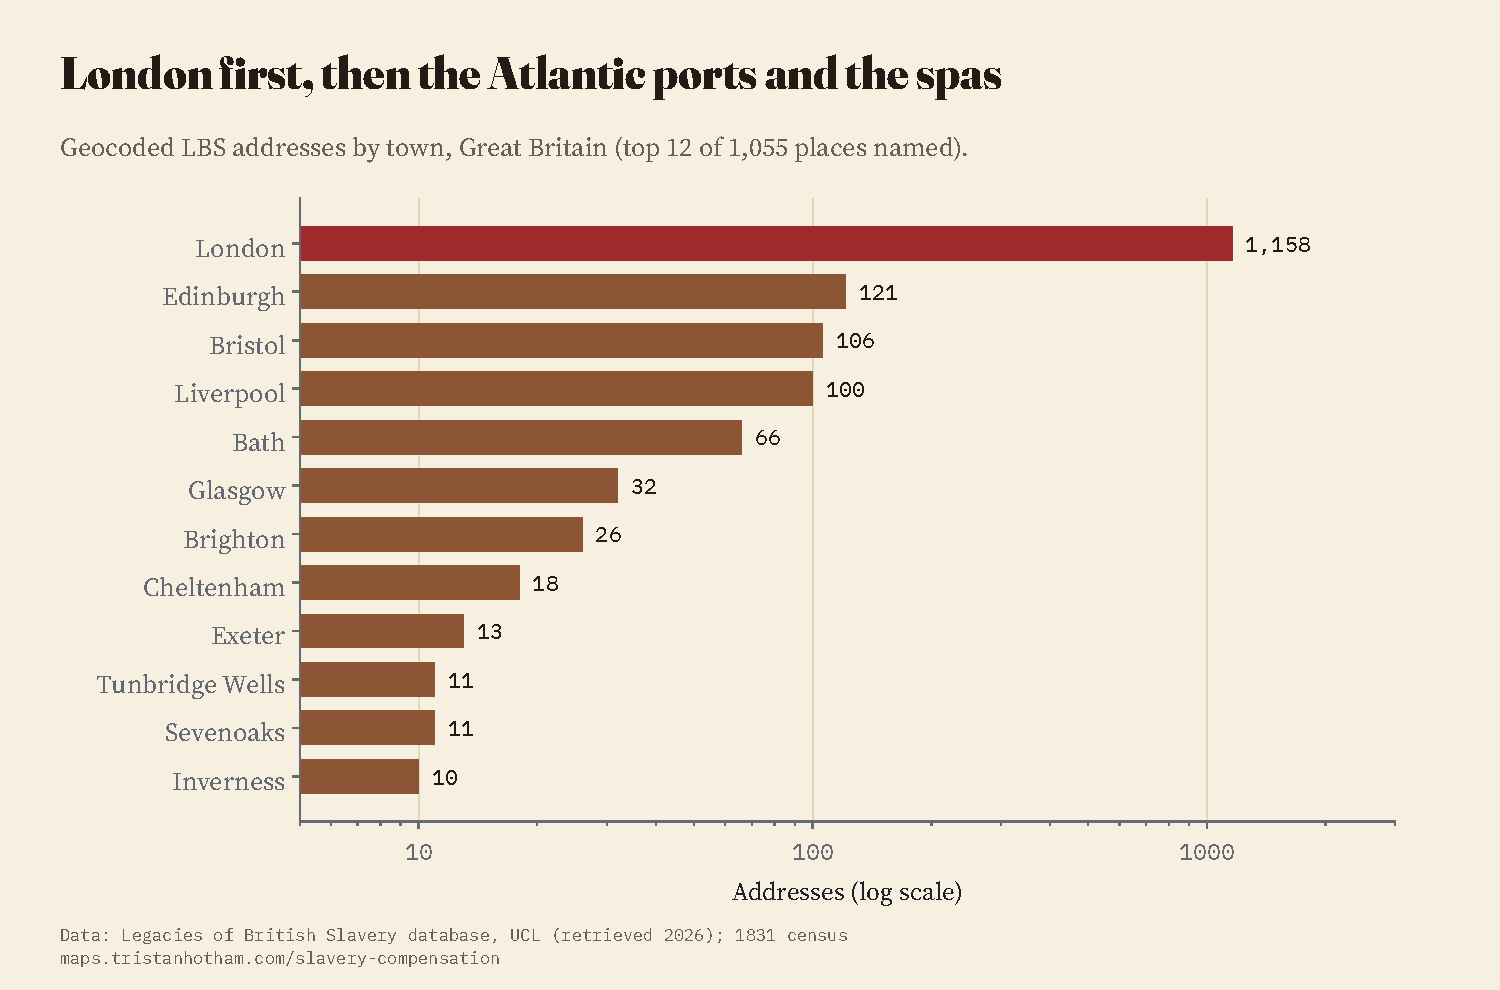
\includegraphics[width=0.8\textwidth]{f_towns.pdf}\caption{Geocoded LBS addresses by town, Great Britain (log scale).}\label{fig:towns}\end{figure}

\begin{figure}[tbp]\centering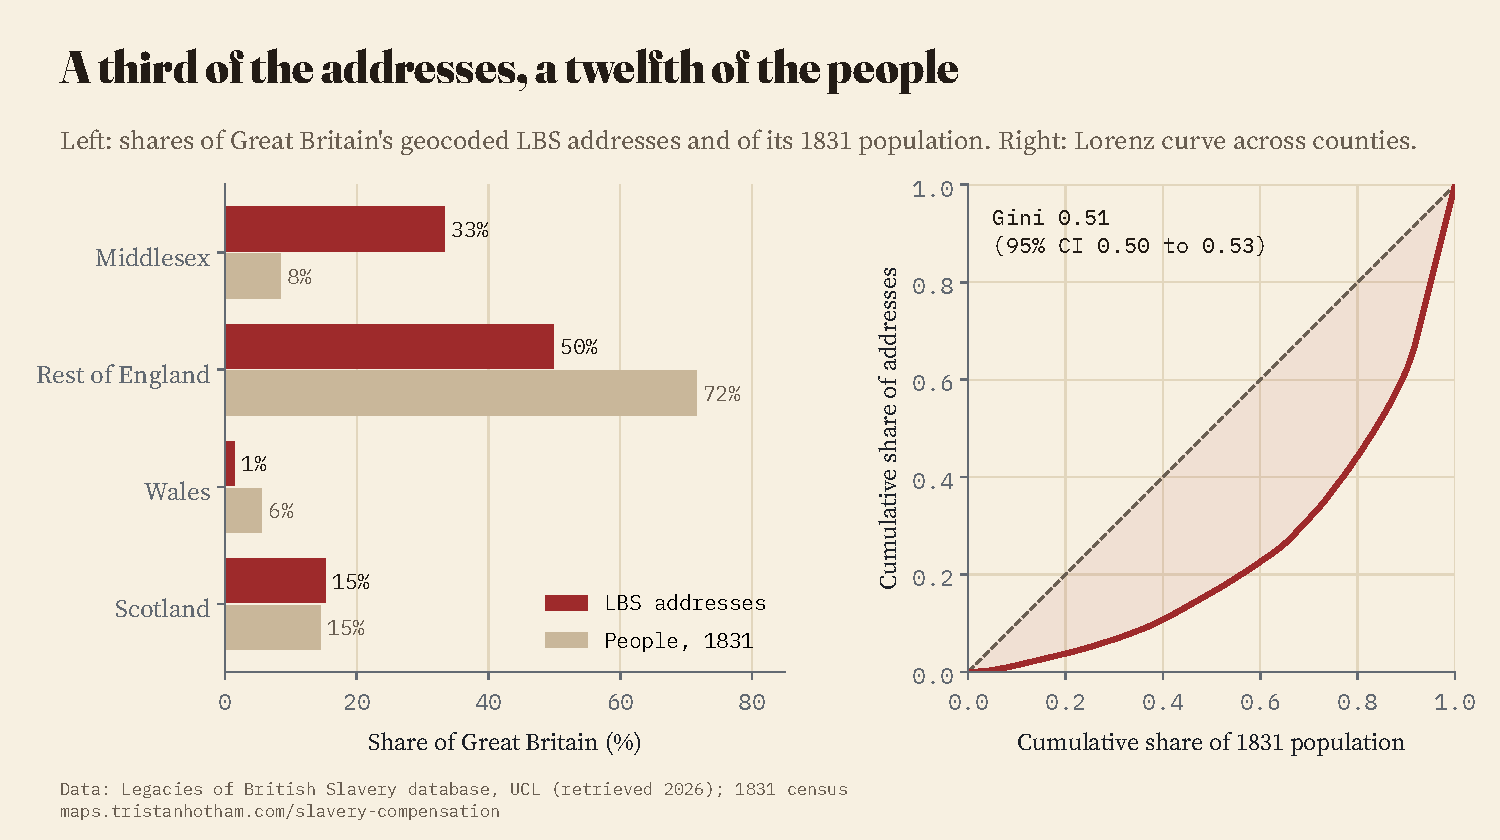
\includegraphics[width=0.85\textwidth]{f_shares.pdf}\caption{Left: shares of geocoded LBS addresses and of 1831 population. Right: Lorenz curve of addresses across counties ordered by rate.}\label{fig:shares}\end{figure}

\subsection{Per head}
Great Britain had 1.96 geocoded addresses per 10,000 people in 1831 (Table~\ref{tab:top}, Figure~\ref{fig:counties}). Among counties with at least 10,000 people the highest rates are Middlesex (7.83), Midlothian (5.65), Moray (5.51, from 19 addresses) and Gloucestershire (4.10); Nairnshire, with 9,354 people, has 8 addresses (8.55). The lowest are in Wales and the English Midlands. Scotland's rate (2.06) is almost the same as England's (2.04), in line with the work on Scotland's deep involvement in Caribbean slavery \citep{devine2015,mullen2022}; Wales's is a quarter of either (0.51). The industrial counties had low rates despite their ports: Lancashire 1.11 and Lanarkshire 1.36, with populations swollen by industry, and Yorkshire 0.47.

\begin{table}[tbp]\centering\small\caption{The 15 historic counties (of at least 10,000 people) with the most geocoded LBS addresses per 10,000 people in 1831. Coverage: located share of all addresses in the LBS county table.}\label{tab:top}\begin{tabular}{llrrrrr}\toprule County & Nation & Population 1831 & Addresses & Per 10,000 & People & Coverage \%\\\midrule
Middlesex & England & 1,358,330 & 1,063 & 7.83 & 1,400 & 60\\
Midlothian (Edinburgh) & Scotland & 219,345 & 124 & 5.65 & 156 & 87\\
Moray & Scotland & 34,498 & 19 & 5.51 & 32 & 76\\
Gloucestershire & England & 387,398 & 159 & 4.10 & 371 & 65\\
Sussex & England & 272,644 & 99 & 3.63 & 151 & 75\\
Somerset & England & 403,795 & 133 & 3.29 & 241 & 60\\
Kent & England & 479,558 & 145 & 3.02 & 183 & 70\\
Peeblesshire & Scotland & 10,578 & 3 & 2.84 & 11 & 100\\
Hampshire & England & 313,976 & 89 & 2.83 & 144 & 47\\
Wigtownshire & Scotland & 36,258 & 10 & 2.76 & 9 & 82\\
Stirlingshire & Scotland & 72,621 & 20 & 2.75 & 26 & 54\\
Inverness-shire & Scotland & 94,797 & 26 & 2.74 & 32 & 70\\
Berwickshire & Scotland & 34,048 & 9 & 2.64 & 11 & 64\\
Surrey & England & 486,434 & 126 & 2.59 & 222 & 39\\
Hertfordshire & England & 142,844 & 36 & 2.52 & 52 & 44\\
\midrule Great Britain & & 16,261,183 & 3,187 & 1.96 & 4,004 & 61\\
\bottomrule\end{tabular}\end{table}

\begin{figure}[tbp]\centering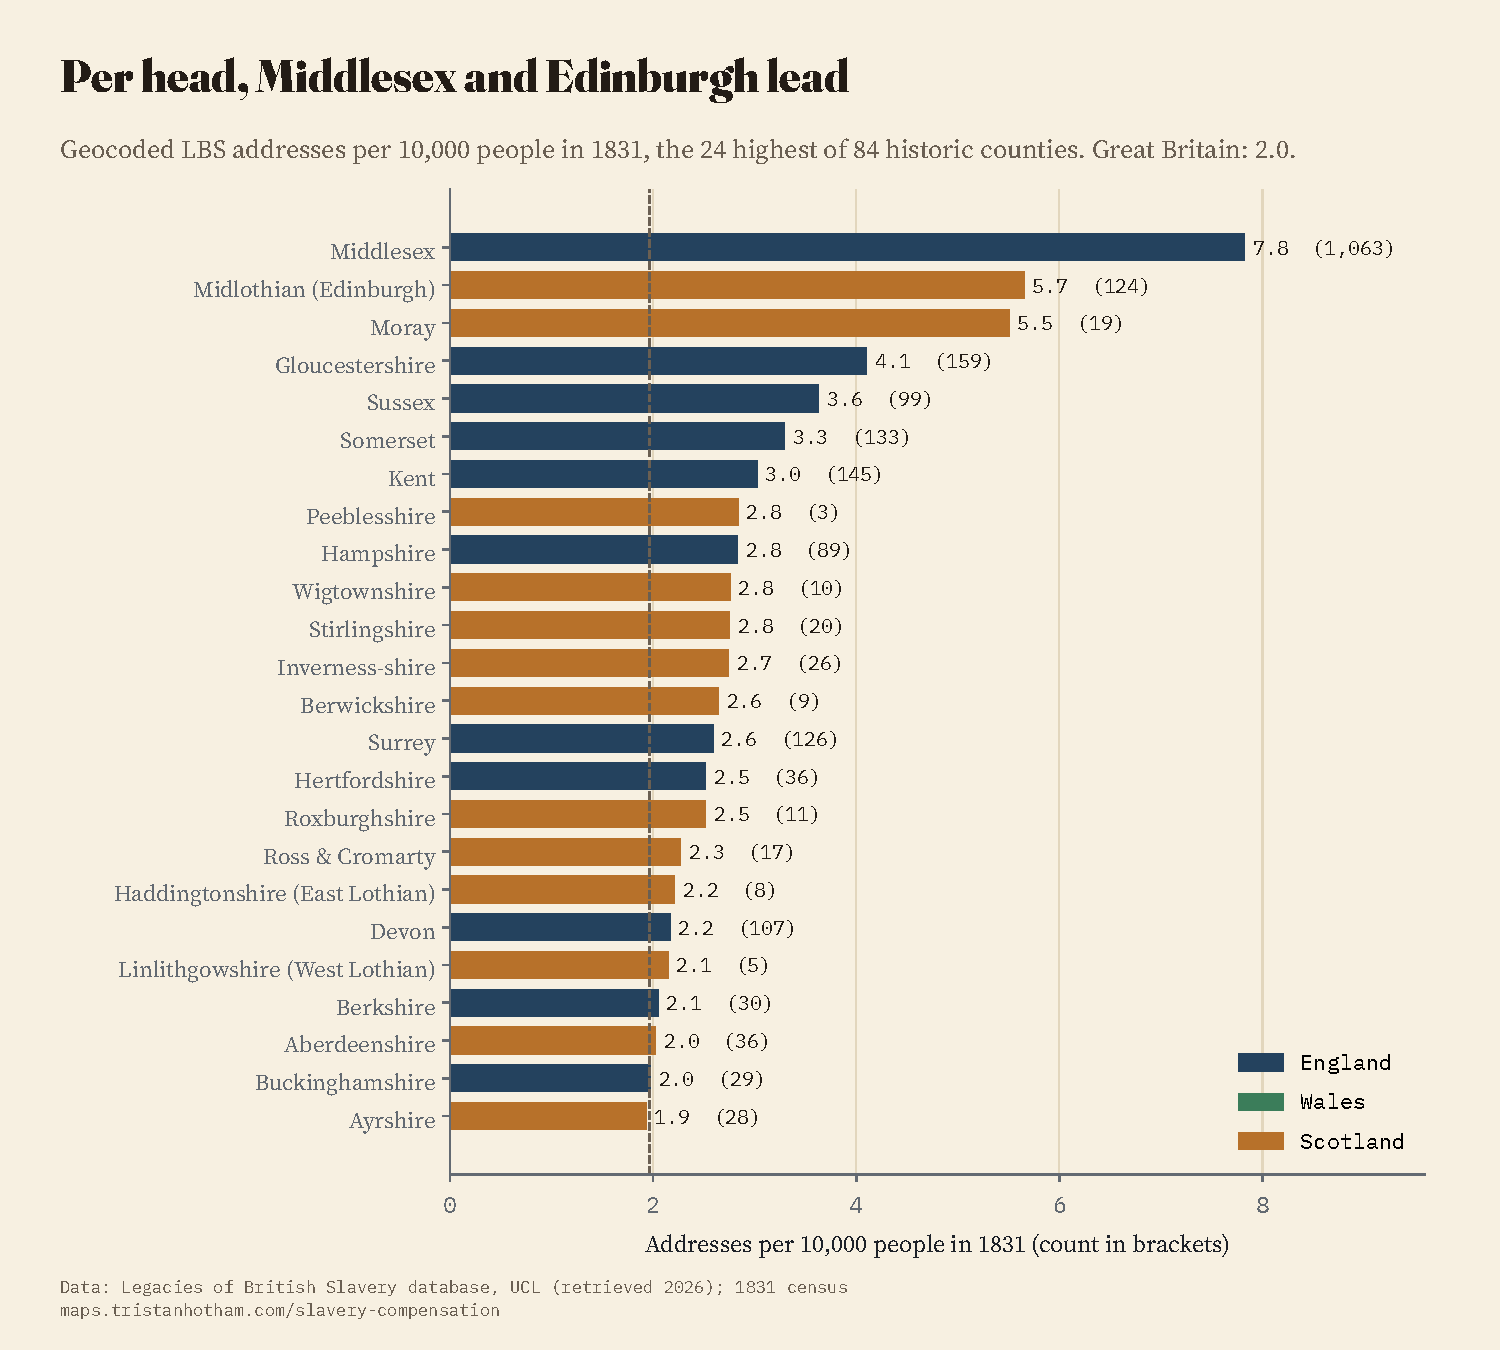
\includegraphics[width=0.8\textwidth]{f_counties.pdf}\caption{Geocoded LBS addresses per 10,000 people in 1831, the 24 highest historic counties of at least 10,000 people (counts in brackets). Dashed line: Great Britain.}\label{fig:counties}\end{figure}

\subsection{Distance from the ports}
Table~\ref{tab:models} gives the main model. Each doubling of the distance from a county's centre to the nearest of the four ports goes with a rate 37\% lower (rate ratio 0.63, 95\% CI 0.54 to 0.75; per unit of log distance 0.52, CI 0.41 to 0.65). The port-county term is not supported: 0.83 (CI 0.44 to 1.57). Once distance is counted, containing a port adds nothing, which is unsurprising given that the port counties are by construction the nearest, and given the low rates of Lancashire and Lanarkshire. H2 is therefore supported for distance and not for the port counties as such. Figure~\ref{fig:distance} shows the counties.

\begin{table}[tbp]\centering\footnotesize\caption{Poisson models of county address counts with offset log population (1831), HC1 standard errors. Distance: rate ratio per doubling of distance to the nearest of the four ports; port: rate ratio for a port county. All models include Wales and Scotland indicators where both vary. 95\% CIs in brackets.}\label{tab:models}\begin{tabular}{p{7.2cm}llr}\toprule Model & Distance (per doubling) & Port county & N\\\midrule
Main: Poisson, geocoded addresses & 0.63 [0.54, 0.75] & 0.83 [0.44, 1.57] & 84\\
Negative binomial & 0.78 [0.67, 0.92] & 1.21 [0.56, 2.61] & 84\\
Linked people (distinct) instead of addresses & 0.68 [0.55, 0.84] & 1.04 [0.44, 2.46] & 84\\
All LBS addresses, located or not & 0.58 [0.49, 0.68] & 0.64 [0.34, 1.18] & 84\\
Middlesex left out & 0.73 [0.62, 0.85] & 0.74 [0.36, 1.53] & 83\\
England only & 0.62 [0.52, 0.74] & 0.91 [0.44, 1.89] & 39\\
Scotland only & 0.92 [0.73, 1.15] & 0.48 [0.21, 1.11] & 32\\
1841 population as the offset & 0.63 [0.53, 0.75] & 0.77 [0.39, 1.53] & 84\\
Named houses only & 0.94 [0.80, 1.11] & 0.56 [0.27, 1.16] & 84\\
Street addresses only & 0.51 [0.42, 0.63] & 1.31 [0.53, 3.23] & 84\\
Exploratory: distance to London instead of the nearest port & 0.74 [0.67, 0.80] & 1.39 [0.90, 2.15] & 84\\
England and Wales only (placebo comparison) & 0.62 [0.52, 0.74] & 0.92 [0.44, 1.90] & 52\\
Placebo: listed great houses (Grade I and II*) & 0.98 [0.82, 1.16] & 0.28 [0.11, 0.73] & 52\\
\bottomrule\end{tabular}\end{table}

\begin{figure}[tbp]\centering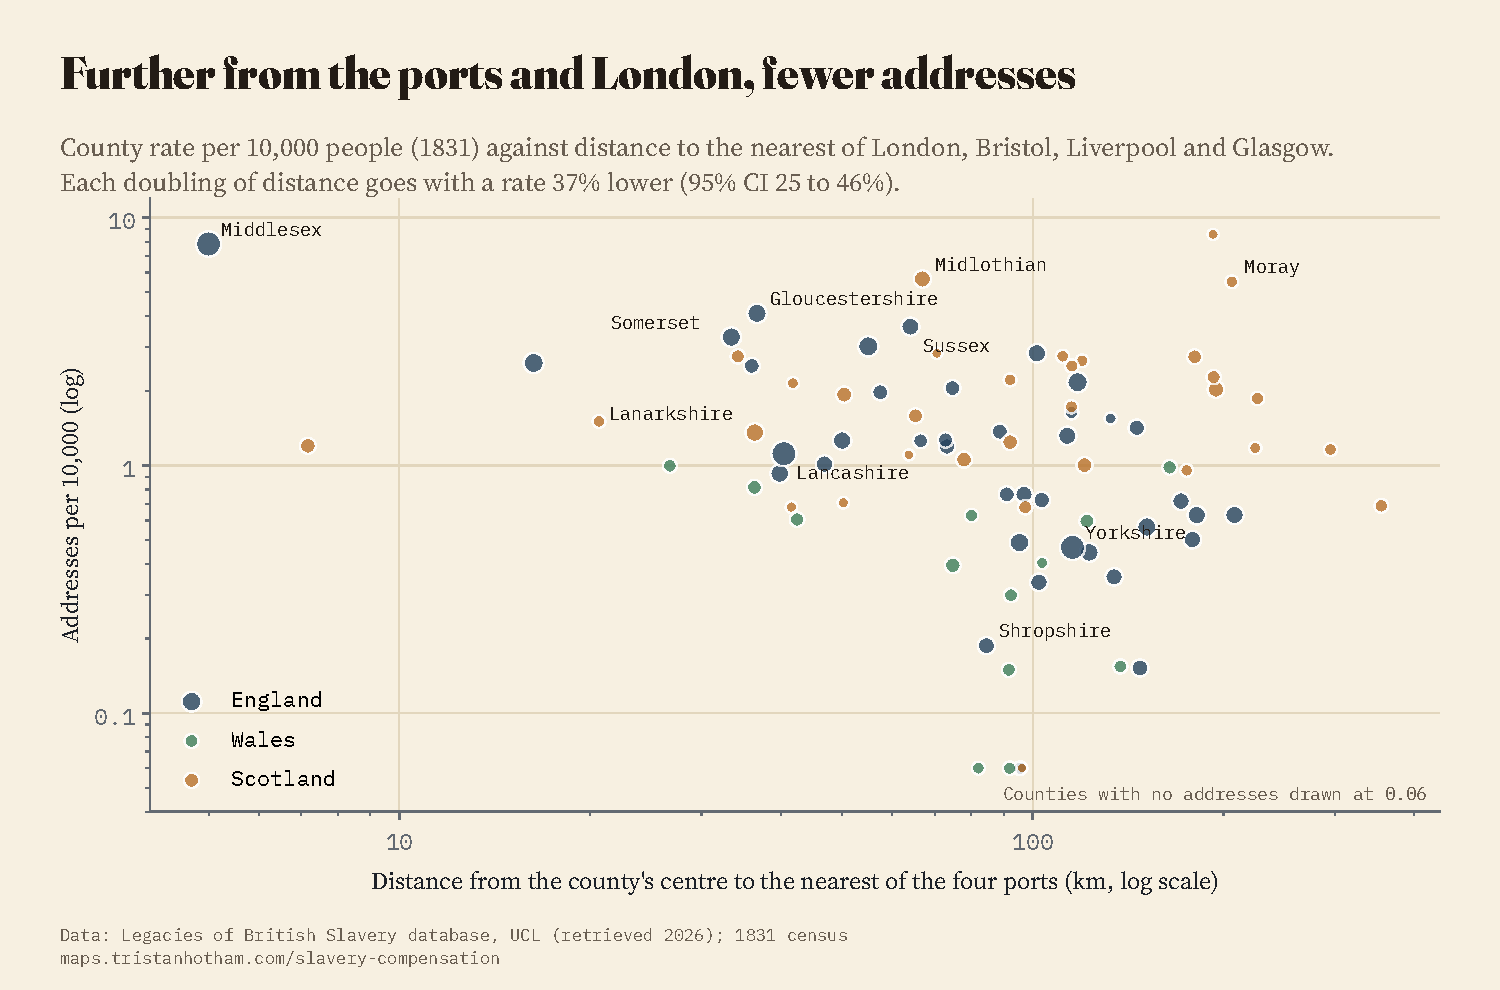
\includegraphics[width=0.85\textwidth]{f_distance.pdf}\caption{County rate per 10,000 people against distance to the nearest of London, Bristol, Liverpool and Glasgow (log scales). Dot size: 1831 population.}\label{fig:distance}\end{figure}

\subsection{Town and country}
In London 89\% of addresses are street addresses (Figure~\ref{fig:forms}, Table~\ref{tab:forms}). Outside London the mix is quite different: 32\% street addresses, 28\% named houses and 39\% records that give only a town, village or parish. Scotland (38\% street, 26\% named houses) and Wales resemble provincial England. Named houses are most often geocoded to the building itself (56\%), settlement-only records almost never (4\%). In the exploratory density check, 21\% of addresses in England and Wales outside London lie in parishes that were dense in 1801. These include 52\% of the street addresses, while 95\% of named houses lie outside them.

\begin{figure}[tbp]\centering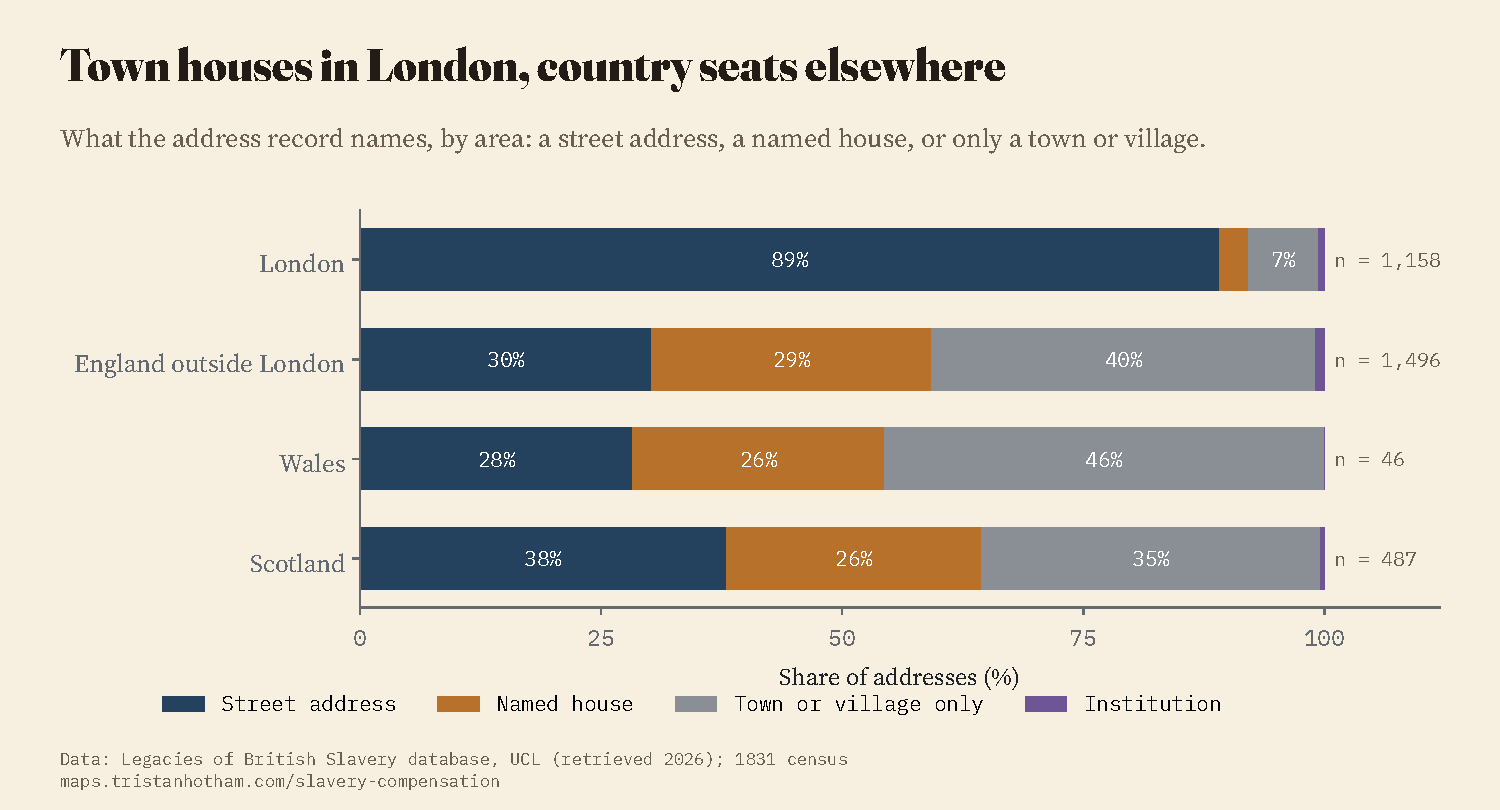
\includegraphics[width=0.85\textwidth]{f_forms.pdf}\caption{Address forms by area.}\label{fig:forms}\end{figure}

\begin{table}[tbp]\centering\small\caption{Address forms by area (percentages of addresses).}\label{tab:forms}\begin{tabular}{lrrrrr}\toprule Area & N & Street & Named house & Settlement only & Institution\\\midrule
London & 1,158 & 89.1 & 3.0 & 7.3 & 0.6\\
England outside London & 1,496 & 30.3 & 28.9 & 39.9 & 0.9\\
Wales & 46 & 28.3 & 26.1 & 45.7 & 0.0\\
Scotland & 487 & 38.0 & 26.5 & 35.1 & 0.4\\
\bottomrule\end{tabular}\end{table}

\subsection{Country houses and listed buildings}
Of the 553 country-house candidates, 267 (48.3\%) match a listed building today: 47\% in England, 53\% in Scotland and 6 of 12 in Wales (Figure~\ref{fig:listed}). The match rate is much higher where the address was geocoded to the building (63\%) than where it was placed at a street (14\%) or only an area (36\%), as one would expect if poor geocodes hide true matches. Corrected for the hand check, the share is 44\% (interval 38 to 49\%). Of the matched houses, 62 are in the top grade (Grade I or Category A) and 101 in the second (Grade II* or Category B). The rest of the candidates include houses since demolished, houses never listed, and records whose name or place the rule could not resolve.

By county in England and Wales there are 8.3 country-house candidates per 100 listed great houses overall. The ratio is highest in Sussex, Lancashire and Hampshire (Table~\ref{tab:listedc}), and across the 51 counties with at least 10 listed great houses it rises with the county address rate (Spearman's $\rho$ = 0.53, $p$ < 0.001), as H4 expected; the two measures share their numerator in part, so the correlation is descriptive.

\begin{figure}[tbp]\centering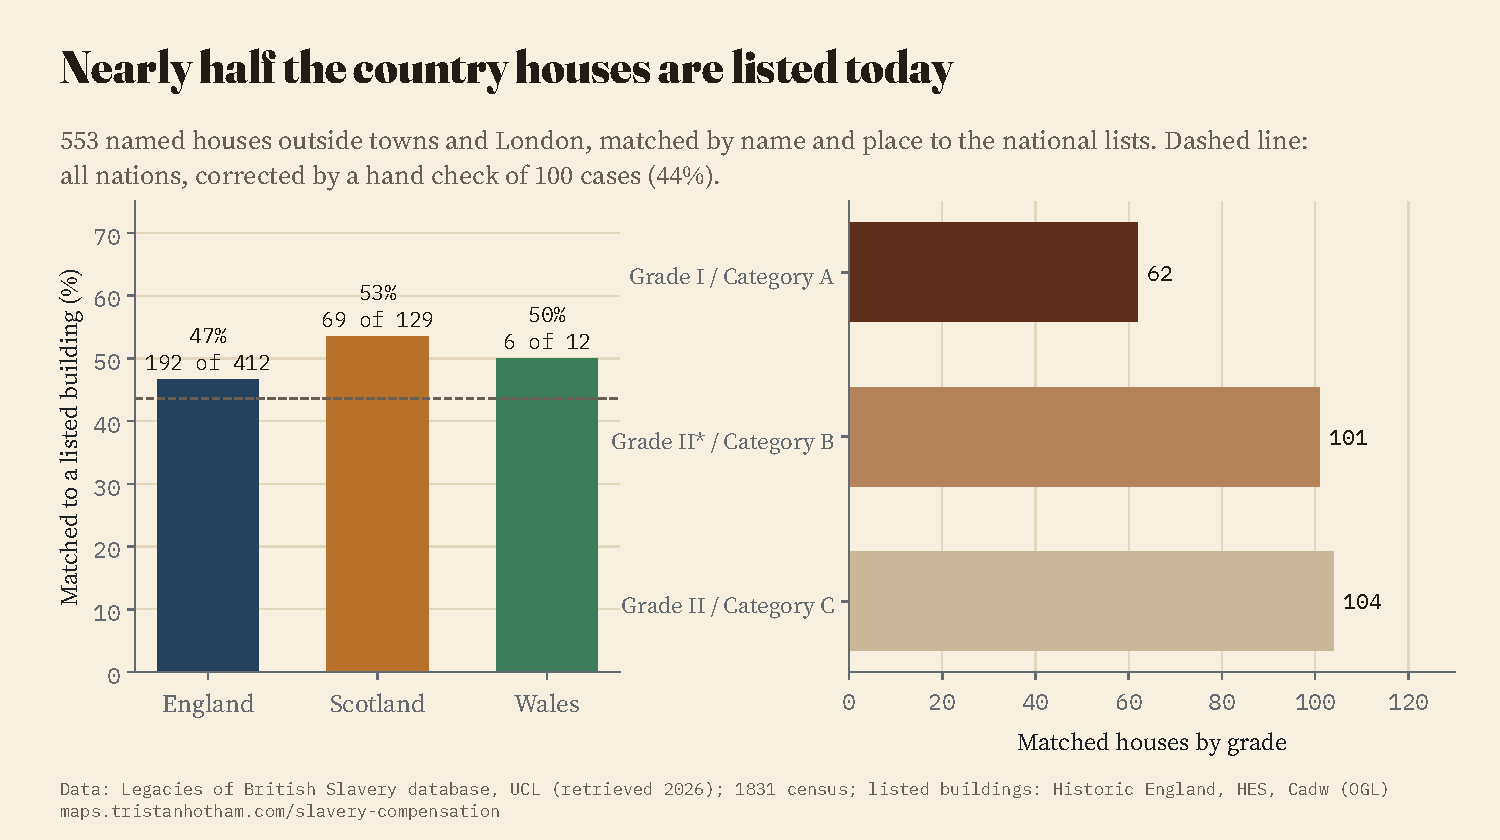
\includegraphics[width=0.85\textwidth]{f_listed.pdf}\caption{Country-house candidates matched to listed buildings, by nation, and the grades of the matched entries.}\label{fig:listed}\end{figure}

\begin{table}[tbp]\centering\small\caption{Country-house candidates per 100 listed great houses (Grade I and II*), England and Wales, the ten highest counties with at least 10 listed great houses.}\label{tab:listedc}\begin{tabular}{lrrrrr}\toprule County & Great houses & Candidates & Matched & Per 100 & Addresses per 10,000\\\midrule
Sussex & 147 & 32 & 10 & 21.8 & 3.63\\
Lancashire & 150 & 31 & 9 & 20.7 & 1.11\\
Hampshire & 179 & 35 & 10 & 19.6 & 2.83\\
Denbighshire & 27 & 5 & 3 & 18.5 & 0.60\\
Buckinghamshire & 87 & 14 & 8 & 16.1 & 1.97\\
Devon & 183 & 29 & 10 & 15.8 & 2.17\\
Cumberland & 53 & 8 & 2 & 15.1 & 1.42\\
Kent & 238 & 33 & 14 & 13.9 & 3.02\\
Herefordshire & 54 & 7 & 3 & 13.0 & 1.27\\
Hertfordshire & 111 & 13 & 6 & 11.7 & 2.52\\
\bottomrule\end{tabular}\end{table}

\section{Robustness}\label{sec:robust}
Figure~\ref{fig:robust} and Table~\ref{tab:models} give every planned check. The distance gradient survives the negative binomial model (0.78 per doubling, CI 0.67 to 0.92), though it is weaker, as expected when the large Middlesex count has less leverage. It holds with linked people (0.68), with all LBS addresses including the unlocated (0.58), without Middlesex (0.73), in England alone (0.62) and with the 1841 population (0.63). Across the 20 leave-one-region-out runs the estimate ranges from 0.60 to 0.78 per doubling, but when the LBS South-East region is left out (it includes Middlesex, Surrey, Kent, Sussex, Essex and Hertfordshire) the interval includes 1 (0.78, CI 0.58 to 1.03). I therefore do not call the result robust in the strict sense: the gradient depends on London and the counties around it. Within Scotland alone there is no clear gradient (0.92, CI 0.73 to 1.15).

Two checks say what kind of pattern this is. Street addresses follow the gradient strongly (0.51 per doubling); named houses do not (0.94, CI 0.80 to 1.11). And the placebo outcome, listed great houses in England and Wales, shows no gradient (0.98, CI 0.82 to 1.16), against 0.62 for LBS addresses in the same counties. The geography of the addresses is not just the geography of old landed wealth.

Exploratory: replacing distance to the nearest port with distance to London alone fits the counts better (AIC 1238 against 1374; 0.74 per doubling), so most of the gradient is a gradient from London. The geocoded share varies by county, from 17\% (Shropshire) to 100\% (Durham) among the 58 counties with at least 10 LBS addresses (median 63\%), but it is unrelated to the county rate (Spearman's $\rho$ = 0.08).

\begin{figure}[tbp]\centering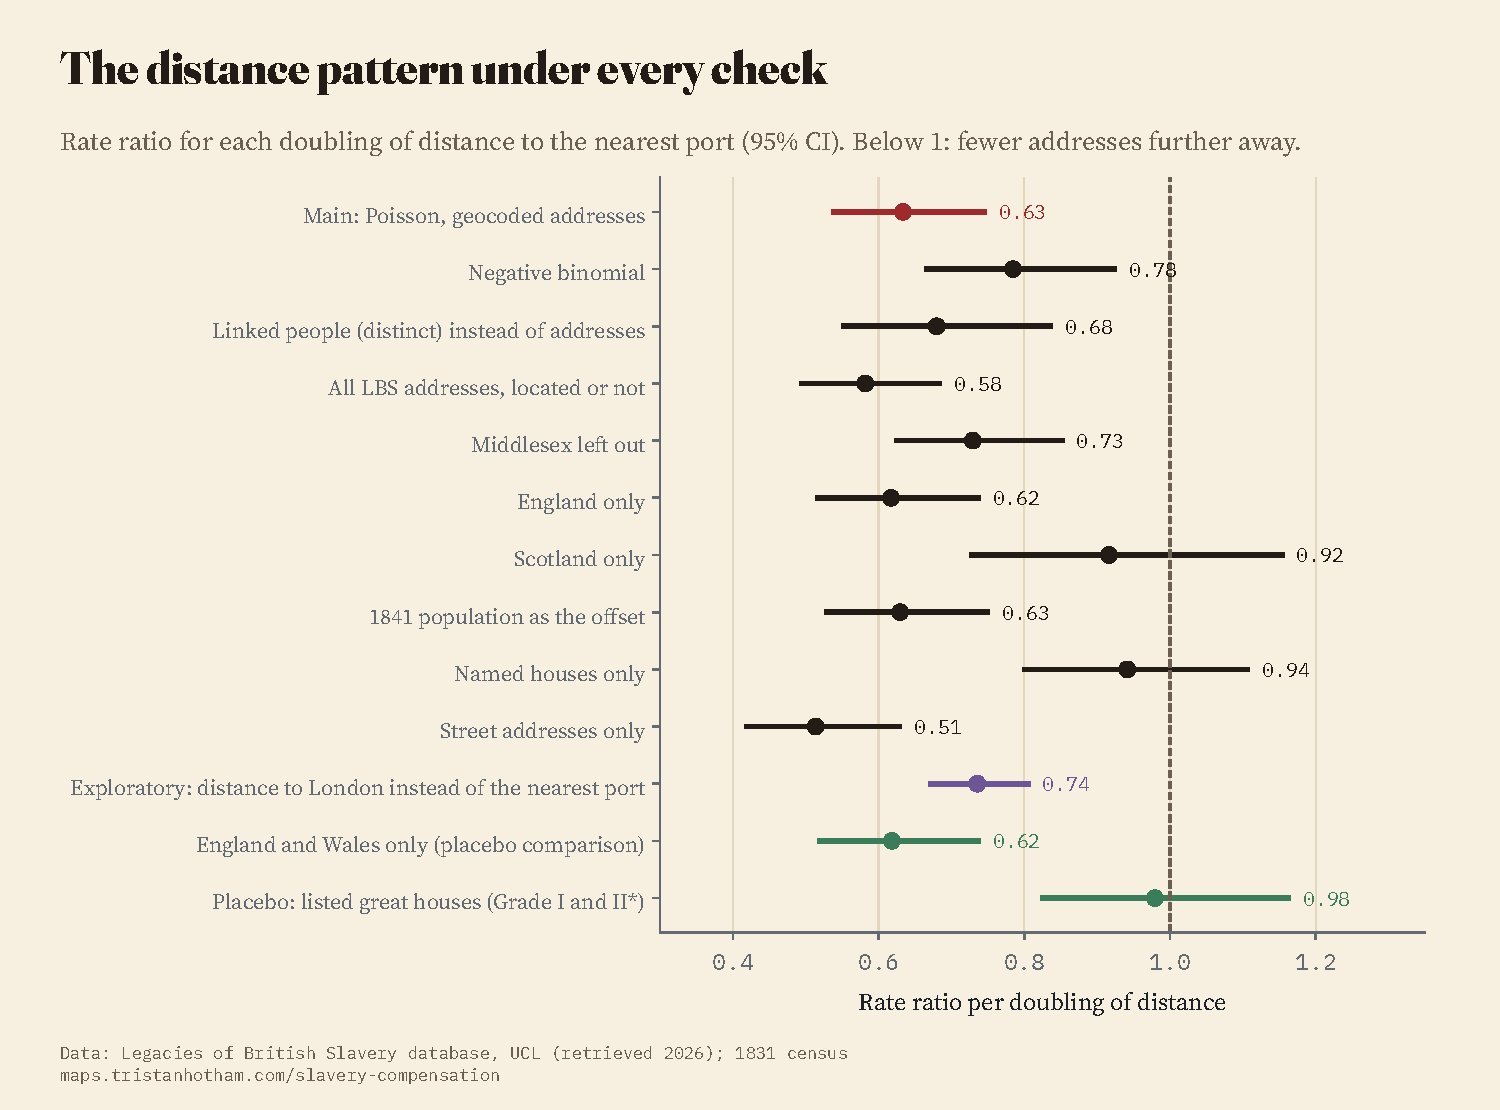
\includegraphics[width=0.85\textwidth]{f_robust.pdf}\caption{Rate ratio per doubling of distance to the nearest port under every check (95\% CI). Green: placebo comparison; purple: exploratory.}\label{fig:robust}\end{figure}

\section{Discussion}\label{sec:disc}
\subsection{What the pattern says}
The addresses of the people linked to slave-ownership at abolition were, above all, metropolitan. A third of them are in Middlesex, which had a twelfth of Britain's people, and the next densest places are Edinburgh, the Atlantic ports and the resort towns of the south and west. This fits the historical work on absentee ownership and the City \citep{draper2007,draper2010,draper2008}, and the per-capita view makes it concrete for the whole of Great Britain. The parity of Scotland and England per head fits the recovery of Scotland's slavery past by \citet{devine2015} and \citet{mullen2022}; the low Welsh rate is a finding that deserves archival work rather than speculation here.

The distance pattern is better read as a London pattern than an Atlantic one. Counties nearer the four ports had more addresses per head, but the port counties themselves did not, distance to London fits better, and the gradient fades without the South-East. It is carried by town addresses. Country houses, by contrast, are scattered with little regard to distance, much as listed great houses are. One reading, consistent with the literature on country houses and slavery \citep{dresser2013,seymour1998,smith2006}, is that the money that reached the countryside did so by joining an older landed geography rather than by following the trade routes. The data show the association, not the mechanism.

\subsection{What survives}
Somewhere between 38\% and 49\% of the country-house addresses can be found on today's lists of listed buildings, with 62 in the top grade. These are buildings that the state has chosen to protect for their architectural or historic interest. The National Trust's review \citep{huxtable2020} and the English Heritage volume edited by \citet{dresser2013} have begun to tell the stories of some of them; the matches released with this paper could help heritage bodies and local historians find others. They are matches by name and place only, and each needs checking against the LBS record and the list entry before anyone relies on it.

\subsection{Implications for research and for heritage}
For historians, the main lesson of the per-capita view is that the national picture is dominated by one metropolitan region, and that outside it the addresses are spread widely and thinly, with a distinct cluster in the resort and spa towns of the south and west and in Edinburgh. Work on provincial places, including the Welsh counties with few or no located addresses, should check whether the low counts reflect fewer people or fewer located addresses: the coverage data released with this paper make that check possible county by county. For quantitative work that uses the LBS data as an explanatory variable, the results suggest caution in two directions. Rates per head vary by a factor of more than ten between counties, but much of that variation is carried by street addresses near London, so models that treat all addresses alike may mix a metropolitan pattern with a landed one. And the addresses are residences over a lifetime, not the place where compensation was received or spent.

For heritage bodies, the listed-building match offers a starting list rather than a finding. A match says that a house of that name stands, listed, near the recorded address. It does not say that the listed building is the one in which the person lived (houses were rebuilt and renamed), nor anything about how much of its fabric was paid for with slavery wealth. Used with the LBS records and the list entries, it could help to identify houses whose list descriptions say nothing about these connections. Whether and how such connections are presented is a matter for those bodies and the communities they serve, and the people descended from the enslaved have the first claim to be heard in it \citep{beckles2013}.

\subsection{Limitations}
The limits are those the LBS team state. The address file is a search tool. Only the located addresses are here, and the located share varies by county, although not in a way related to the rates. Addresses are where people lived at some time, often with no dates; a person can have several, and an address several people, so counts of addresses are not counts of people or of money. A third of the geocodes are only a town or parish. County outlines for England and Wales on the maps are approximations rebuilt from parish centroids (they are never used to count), and Scotland's counties are shown as points. The listed-building match is approximate, with the error rates given. The county regressions have 84 units and are associations only; the paper makes no causal claim.

There is also a limit of a different kind. The records were made to value property and to pay owners. They describe the people who were paid, and by their nature they do not describe the people whose freedom was the occasion for the payment, or the lives that were lost; the LBS team note that the database does not hold systematic information on the enslaved. A map of owners' addresses is a map of where one side of that relationship lived. It is not a measure of the harm done, and it should not be read as one.

\section{Conclusion}\label{sec:conc}
The compensation of 1834 went to slave-owners, and the Legacies of British Slavery database shows where many of them lived. Set against the 1831 census, the located addresses are concentrated in London and the South-East, in Edinburgh, the Atlantic ports and the resort towns; Scotland matches England per head and Wales lags far behind. Addresses thin out with distance from the ports, but that gradient is mainly a pull towards London and is carried by town houses, while country seats follow an older landed geography. Nearly half of the country houses linked to these people survive as listed buildings. All of this describes a database built for searching, not counting, and the analysis should be revisited as the LBS team locate more addresses.

\section*{Data availability statement}
Data and code: Zenodo DOI https://doi.org/10.5281/zenodo.24113858. The repository holds county and town counts, unnamed address points with LBS identifiers but no names, the listed-building matches and hand check, and the code. The LBS address file itself is not redistributed; it is available on the LBS website.

\section*{AI statement}
I wrote the text, with drafting and editing assistance from Claude (Anthropic), which also helped prepare the analysis code. I reviewed and checked all text and results.

\begin{thebibliography}{99}
\bibitem[Baker(2024)]{baker2024} Baker, J. (2024) 1833 Slavery Abolition Act: the long road to emancipation in the British West Indies. \textit{The History of Parliament} (blog), 28 August 2024. https://historyofparliament.com/2024/08/28/1833-slavery-abolition-act
\bibitem[Beckles(2013)]{beckles2013} Beckles, H. McD. (2013) \textit{Britain's Black Debt: Reparations for Caribbean Slavery and Native Genocide}. Kingston: University of the West Indies Press.
\bibitem[Butler(1995)]{butler1995} Butler, K. M. (1995) \textit{The Economics of Emancipation: Jamaica and Barbados, 1823 to 1843}. Chapel Hill: University of North Carolina Press.
\bibitem[Cameron and Trivedi(2013)]{cameron2013} Cameron, A. C. and Trivedi, P. K. (2013) \textit{Regression Analysis of Count Data}, 2nd edn. Cambridge: Cambridge University Press.
\bibitem[Caprettini and Voth(2020)]{caprettini2020} Caprettini, B. and Voth, H.-J. (2020) Rage against the machines: labor-saving technology and unrest in industrializing England. \textit{American Economic Review: Insights} 2(3), 305 to 320. doi:10.1257/aeri.20190385. Replication data: openICPSR E117044, CC BY 4.0.
\bibitem[Census of Great Britain(1852)]{census1851} Census of Great Britain, 1851 (1852) \textit{Population Tables I. Numbers of the Inhabitants in the Years 1801, 1811, 1821, 1831, 1841 and 1851}, Vol. I. London: HMSO. Tables XXX and X.
\bibitem[Devine(2015)]{devine2015} Devine, T. M., ed. (2015) \textit{Recovering Scotland's Slavery Past: The Caribbean Connection}. Edinburgh: Edinburgh University Press.
\bibitem[Ditto Books(2026)]{ditto2026} Ditto Books (2026) Census population 1801 to 1851 (county totals transcribed from the 1851 census Population Tables). https://dittobooks.co.uk/extras/census/census-population-1801-1851, retrieved 2026.
\bibitem[Donington(2019)]{donington2019} Donington, K. (2019) \textit{The Bonds of Family: Slavery, Commerce and Culture in the British Atlantic World}. Manchester: Manchester University Press.
\bibitem[Draper(2007)]{draper2007} Draper, N. (2007) ``Possessing slaves'': ownership, compensation and metropolitan society in Britain at the time of emancipation, 1834 to 1840. \textit{History Workshop Journal} 64, 74 to 102.
\bibitem[Draper(2008)]{draper2008} Draper, N. (2008) The City of London and slavery: evidence from the first dock companies, 1795 to 1800. \textit{Economic History Review} 61(2), 432 to 466.
\bibitem[Draper(2010)]{draper2010} Draper, N. (2010) \textit{The Price of Emancipation: Slave-Ownership, Compensation and British Society at the End of Slavery}. Cambridge: Cambridge University Press.
\bibitem[Dresser(2001)]{dresser2001} Dresser, M. (2001) \textit{Slavery Obscured: The Social History of the Slave Trade in an English Provincial Port}. London: Continuum.
\bibitem[Dresser and Hann(2013)]{dresser2013} Dresser, M. and Hann, A., eds (2013) \textit{Slavery and the British Country House}. Swindon: English Heritage.
\bibitem[Eltis and Engerman(2000)]{eltis2000} Eltis, D. and Engerman, S. L. (2000) The importance of slavery and the slave trade to industrializing Britain. \textit{Journal of Economic History} 60(1), 123 to 144.
\bibitem[Hall et al.(2014)]{hall2014} Hall, C., Draper, N., McClelland, K., Donington, K. and Lang, R. (2014) \textit{Legacies of British Slave-ownership: Colonial Slavery and the Formation of Victorian Britain}. Cambridge: Cambridge University Press.
\bibitem[Heblich et al.(2022)]{heblich2022} Heblich, S., Redding, S. J. and Voth, H.-J. (2022) Slavery and the British Industrial Revolution. NBER Working Paper 30451. doi:10.3386/w30451.
\bibitem[Holt(1992)]{holt1992} Holt, T. C. (1992) \textit{The Problem of Freedom: Race, Labor, and Politics in Jamaica and Britain, 1832 to 1938}. Baltimore: Johns Hopkins University Press.
\bibitem[Hotham(2026)]{hotham2026listed} Hotham, T. (2026) \textit{The Listed Kingdom: every listed building in the United Kingdom by grade, type, date of listing and date of building}. Zenodo. doi:10.5281/zenodo.23761429.
\bibitem[Huxtable et al.(2020)]{huxtable2020} Huxtable, S.-A., Fowler, C., Kefalas, C. and Slocombe, E., eds (2020) \textit{Interim Report on the Connections between Colonialism and Properties now in the Care of the National Trust, Including Links with Historic Slavery}. Swindon: National Trust.
\bibitem[Inikori(2002)]{inikori2002} Inikori, J. E. (2002) \textit{Africans and the Industrial Revolution in England: A Study in International Trade and Economic Development}. Cambridge: Cambridge University Press.
\bibitem[Lambert(2005)]{lambert2005} Lambert, D. (2005) \textit{White Creole Culture, Politics and Identity during the Age of Abolition}. Cambridge: Cambridge University Press.
\bibitem[LBS(2026a)]{lbs2026details} Legacies of British Slavery (2026a) The database: project details. Centre for the Study of the Legacies of British Slavery, UCL. https://lbs.ucl.ac.uk/lbs/project/details, retrieved 2026.
\bibitem[LBS(2026b)]{lbs2026maps} Legacies of British Slavery (2026b) Maps, and the map address data for Britain. Centre for the Study of the Legacies of British Slavery, UCL. https://lbs.ucl.ac.uk/lbs/maps/, retrieved 2026.
\bibitem[Mullen(2021)]{mullen2021} Mullen, S. (2021) British universities and transatlantic slavery: the University of Glasgow case. \textit{History Workshop Journal} 91(1), 210 to 233. doi:10.1093/hwj/dbaa035.
\bibitem[Mullen(2022)]{mullen2022} Mullen, S. (2022) \textit{The Glasgow Sugar Aristocracy: Scotland and Caribbean Slavery, 1775 to 1838}. London: University of London Press.
\bibitem[Richardson et al.(2007)]{richardson2007} Richardson, D., Schwarz, S. and Tibbles, A., eds (2007) \textit{Liverpool and Transatlantic Slavery}. Liverpool: Liverpool University Press.
\bibitem[Santos Silva and Tenreyro(2006)]{santossilva2006} Santos Silva, J. M. C. and Tenreyro, S. (2006) The log of gravity. \textit{Review of Economics and Statistics} 88(4), 641 to 658. doi:10.1162/rest.88.4.641.
\bibitem[Seymour et al.(1998)]{seymour1998} Seymour, S., Daniels, S. and Watkins, C. (1998) Estate and empire: Sir George Cornewall's management of Moccas, Herefordshire and La Taste, Grenada, 1771 to 1819. \textit{Journal of Historical Geography} 24(3), 313 to 351. doi:10.1006/jhge.1998.0089.
\bibitem[Smith(2006)]{smith2006} Smith, S. D. (2006) \textit{Slavery, Family, and Gentry Capitalism in the British Atlantic: The World of the Lascelles, 1648 to 1834}. Cambridge: Cambridge University Press.
\bibitem[Vision of Britain(2026)]{vob2026} A Vision of Britain through Time (2026) Census of Great Britain, 1841, Enumeration Abstract: Area, houses and persons. University of Portsmouth. \url{https://www.visionofbritain.org.uk/census/GB1841ABS_1/3}, retrieved 2026.
\bibitem[Williams(1944)]{williams1944} Williams, E. (1944) \textit{Capitalism and Slavery}. Chapel Hill: University of North Carolina Press.
\end{thebibliography}

\appendix
\section{Appendix: full tables and data construction}
{\footnotesize\begin{longtable}{llrrrrrr}\caption{All historic counties. E England, W Wales, S Scotland. All: all addresses in the LBS county table, located or not. Port km: distance from the county centre to the nearest of the four ports.}\label{tab:appx}\\\toprule County & & Pop. 1831 & Addresses & Per 10,000 & People & All & Port km\\\midrule\endfirsthead\toprule County & & Pop. 1831 & Addresses & Per 10,000 & People & All & Port km\\\midrule\endhead
Bedfordshire & E & 95,483 & 12 & 1.26 & 17 & 21 & 67\\
Berkshire & E & 146,234 & 30 & 2.05 & 44 & 57 & 75\\
Buckinghamshire & E & 146,977 & 29 & 1.97 & 32 & 63 & 57\\
Cambridgeshire & E & 143,955 & 11 & 0.76 & 18 & 14 & 91\\
Cheshire & E & 334,391 & 31 & 0.93 & 39 & 41 & 40\\
Cornwall & E & 301,306 & 19 & 0.63 & 29 & 27 & 208\\
Cumberland & E & 169,262 & 24 & 1.42 & 28 & 27 & 146\\
Derbyshire & E & 237,170 & 8 & 0.34 & 12 & 11 & 102\\
Devon & E & 493,908 & 107 & 2.17 & 175 & 145 & 118\\
Dorset & E & 159,385 & 19 & 1.19 & 32 & 43 & 73\\
Durham & E & 239,256 & 12 & 0.50 & 8 & 12 & 179\\
Essex & E & 317,507 & 40 & 1.26 & 63 & 99 & 50\\
Gloucestershire & E & 387,398 & 159 & 4.10 & 371 & 248 & 37\\
Hampshire & E & 313,976 & 89 & 2.83 & 144 & 190 & 101\\
Herefordshire & E & 110,617 & 14 & 1.27 & 15 & 22 & 73\\
Hertfordshire & E & 142,844 & 36 & 2.52 & 52 & 81 & 36\\
Huntingdonshire & E & 53,192 & 0 & 0.00 & 0 & 6 & 95\\
Kent & E & 479,558 & 145 & 3.02 & 183 & 208 & 55\\
Lancashire & E & 1,336,854 & 149 & 1.11 & 231 & 190 & 40\\
Leicestershire & E & 197,003 & 3 & 0.15 & 3 & 10 & 148\\
Lincolnshire & E & 317,465 & 20 & 0.63 & 31 & 25 & 182\\
Middlesex & E & 1,358,330 & 1,063 & 7.83 & 1,400 & 1,754 & 4\\
Norfolk & E & 390,054 & 22 & 0.56 & 30 & 31 & 151\\
Northamptonshire & E & 179,336 & 13 & 0.72 & 14 & 24 & 103\\
Northumberland & E & 236,959 & 17 & 0.72 & 34 & 18 & 171\\
Nottinghamshire & E & 225,327 & 8 & 0.36 & 8 & 11 & 134\\
Oxfordshire & E & 153,526 & 21 & 1.37 & 29 & 29 & 89\\
Rutland & E & 19,385 & 3 & 1.55 & 6 & 5 & 133\\
Shropshire & E & 213,518 & 4 & 0.19 & 4 & 23 & 84\\
Somerset & E & 403,795 & 133 & 3.29 & 241 & 221 & 33\\
Staffordshire & E & 409,480 & 20 & 0.49 & 25 & 32 & 95\\
Suffolk & E & 296,317 & 39 & 1.32 & 49 & 59 & 113\\
Surrey & E & 486,434 & 126 & 2.59 & 222 & 319 & 16\\
Sussex & E & 272,644 & 99 & 3.63 & 151 & 133 & 64\\
Warwickshire & E & 336,645 & 15 & 0.45 & 23 & 31 & 123\\
Westmorland & E & 55,041 & 9 & 1.64 & 12 & 8 & 115\\
Wiltshire & E & 237,244 & 24 & 1.01 & 42 & 69 & 47\\
Worcestershire & E & 222,655 & 17 & 0.76 & 21 & 27 & 97\\
Yorkshire & E & 1,371,966 & 64 & 0.47 & 79 & 75 & 116\\
Aberdeenshire & S & 177,657 & 36 & 2.03 & 69 & 46 & 195\\
Argyll & S & 100,973 & 16 & 1.58 & 18 & 24 & 65\\
Ayrshire & S & 145,055 & 28 & 1.93 & 29 & 53 & 50\\
Banffshire & S & 48,337 & 9 & 1.86 & 10 & 12 & 226\\
Berwickshire & S & 34,048 & 9 & 2.64 & 11 & 14 & 120\\
Bute & S & 14,151 & 1 & 0.71 & 1 & 0 & 50\\
Caithness & S & 34,529 & 4 & 1.16 & 7 & 6 & 295\\
Clackmannanshire & S & 14,729 & 1 & 0.68 & 1 & 1 & 42\\
Dumfriesshire & S & 73,770 & 5 & 0.68 & 9 & 23 & 97\\
Dunbartonshire & S & 33,211 & 5 & 1.51 & 9 & 11 & 21\\
Fife & S & 128,839 & 16 & 1.24 & 15 & 21 & 92\\
Forfarshire & S & 139,606 & 14 & 1.00 & 21 & 10 & 121\\
Haddingtonshire (East Lothian) & S & 36,145 & 8 & 2.21 & 10 & 7 & 92\\
Inverness-shire & S & 94,797 & 26 & 2.74 & 32 & 33 & 180\\
Kincardineshire & S & 31,431 & 3 & 0.95 & 5 & 6 & 175\\
Kinross-shire & S & 9,072 & 1 & 1.10 & 1 & 2 & 64\\
Kirkcudbrightshire & S & 40,590 & 7 & 1.72 & 9 & 10 & 115\\
Lanarkshire & S & 316,819 & 43 & 1.36 & 118 & 78 & 36\\
Linlithgowshire (West Lothian) & S & 23,291 & 5 & 2.15 & 7 & 8 & 42\\
Midlothian (Edinburgh) & S & 219,345 & 124 & 5.65 & 156 & 139 & 67\\
Moray & S & 34,498 & 19 & 5.51 & 32 & 25 & 206\\
Nairnshire & S & 9,354 & 8 & 8.55 & 6 & 8 & 193\\
Orkney and Shetland & S & 58,239 & 4 & 0.69 & 6 & 0 & 355\\
Peeblesshire & S & 10,578 & 3 & 2.84 & 11 & 2 & 71\\
Perthshire & S & 142,166 & 15 & 1.06 & 24 & 19 & 78\\
Renfrewshire & S & 133,443 & 16 & 1.20 & 28 & 28 & 7\\
Ross \& Cromarty & S & 74,820 & 17 & 2.27 & 32 & 6 & 193\\
Roxburghshire & S & 43,663 & 11 & 2.52 & 14 & 11 & 115\\
Selkirkshire & S & 6,833 & 0 & 0.00 & 0 & 1 & 96\\
Stirlingshire & S & 72,621 & 20 & 2.75 & 26 & 35 & 34\\
Sutherland & S & 25,518 & 3 & 1.18 & 4 & 5 & 225\\
Wigtownshire & S & 36,258 & 10 & 2.76 & 9 & 11 & 111\\
Anglesey & W & 48,325 & 0 & 0.00 & 0 & 0 & 92\\
Brecknockshire & W & 47,763 & 3 & 0.63 & 4 & 1 & 80\\
Caernarfonshire & W & 66,818 & 2 & 0.30 & 3 & 2 & 92\\
Cardiganshire & W & 64,780 & 1 & 0.15 & 1 & 2 & 138\\
Carmarthenshire & W & 100,740 & 6 & 0.60 & 9 & 7 & 122\\
Denbighshire & W & 82,665 & 5 & 0.60 & 9 & 9 & 42\\
Flintshire & W & 60,244 & 6 & 1.00 & 7 & 9 & 27\\
Glamorgan & W & 126,612 & 5 & 0.39 & 5 & 12 & 75\\
Merionethshire & W & 35,315 & 0 & 0.00 & 0 & 0 & 82\\
Monmouthshire & W & 98,126 & 8 & 0.82 & 11 & 14 & 36\\
Montgomeryshire & W & 66,844 & 1 & 0.15 & 1 & 2 & 92\\
Pembrokeshire & W & 81,425 & 8 & 0.98 & 12 & 14 & 164\\
Radnorshire & W & 24,743 & 1 & 0.40 & 1 & 1 & 103\\
\bottomrule\end{longtable}}
\begin{table}[htbp]\centering\footnotesize\caption{Leave one LBS region out (main model).}\label{tab:loro}\begin{tabular}{p{7.2cm}llr}\toprule Region left out & Distance (per doubling) & Port county & N\\\midrule
Without Argyll and Bute & 0.63 [0.54, 0.74] & 0.82 [0.44, 1.56] & 82\\
Without Central England & 0.63 [0.54, 0.75] & 0.83 [0.44, 1.58] & 78\\
Without Central Scotland & 0.63 [0.53, 0.75] & 0.99 [0.48, 2.04] & 77\\
Without Devon and Cornwall & 0.63 [0.53, 0.74] & 0.83 [0.44, 1.57] & 82\\
Without East Anglia & 0.64 [0.54, 0.75] & 0.83 [0.44, 1.57] & 81\\
Without East Midlands & 0.64 [0.54, 0.76] & 0.83 [0.44, 1.59] & 79\\
Without Highlands \& Islands & 0.63 [0.53, 0.74] & 0.82 [0.43, 1.56] & 80\\
Without Mid-Wales & 0.63 [0.54, 0.75] & 0.83 [0.44, 1.57] & 80\\
Without North Wales & 0.63 [0.54, 0.75] & 0.83 [0.44, 1.57] & 79\\
Without North-East Scotland & 0.62 [0.53, 0.73] & 0.81 [0.42, 1.53] & 74\\
Without North-West England & 0.68 [0.57, 0.81] & 1.11 [0.56, 2.22] & 82\\
Without Northern England & 0.63 [0.54, 0.75] & 0.83 [0.44, 1.57] & 80\\
Without Northern Isles & 0.63 [0.54, 0.75] & 0.83 [0.44, 1.57] & 83\\
Without South Wales & 0.63 [0.54, 0.74] & 0.82 [0.44, 1.56] & 80\\
Without South-East England & 0.78 [0.58, 1.03] & 0.89 [0.37, 2.12] & 78\\
Without South-West England & 0.60 [0.52, 0.70] & 0.68 [0.40, 1.16] & 81\\
Without Southern Scotland & 0.63 [0.54, 0.74] & 0.82 [0.43, 1.57] & 76\\
Without Wessex & 0.63 [0.53, 0.74] & 0.83 [0.44, 1.57] & 82\\
Without West Midlands & 0.64 [0.54, 0.76] & 0.82 [0.43, 1.55] & 79\\
Without Yorkshire & 0.65 [0.55, 0.76] & 0.83 [0.44, 1.58] & 83\\
\bottomrule\end{tabular}\end{table}

\textbf{Decisions made by hand.} County spellings and modern names were mapped to historic counties in \texttt{code/rules.py}; two Scottish rows without a county were placed from the place named (Isle of Lewis in Ross and Cromarty; Kirkmaiden in Wigtownshire) and two ``Galloway'' rows by longitude either side of the Cree. Address forms come from text rules in the same file; reading a random sample of 45 named houses and 45 street addresses by eye found the forms right with a few exceptions (for example suburbs given only by name, such as Wavertree, classed as named houses). The listed-building matching rule and the hand check are in \texttt{code/rules.py} and \texttt{code/handcheck.py}; the 100 judged cases are in \texttt{data/listed\_handcheck.csv}. No county, address or match was dropped for a reason related to the outcomes.

\textbf{Software.} Python 3 with pandas, numpy, geopandas, shapely, scipy, statsmodels, rapidfuzz and matplotlib; xelatex. All code is in the data and code archive.

\end{document}
